\documentclass[12pt]{article}

\usepackage{amsmath}
\usepackage{graphicx}
\usepackage{subfigure}
\usepackage{float}
\usepackage{ulem}
\usepackage{bm}

\usepackage{anysize}

\marginsize{2cm}{2cm}{0.9cm}{1.8cm}
\usepackage[framed,numbered,autolinebreaks,useliterate]{mcode}
\usepackage{listings}
\lstset{language=Matlab}
\lstset{breaklines}
\lstset{extendedchars=false}

\title{Machine Learning/Pattern Recognition\\  \begin{Large} Homework \#3 \end{Large} }
\author{Jiyu Tian}
\date{}


\begin{document}

\maketitle
%%---------------------------------------------------------------
%% Problem 1
%%---------------------------------------------------------------
\section{Problem 3.1}
\large{\textbf{Solution:}}\\
(a) The maximum likelihood estimates for $\bm{\mu}$ and $\bm{\Sigma}$ are given by:
\begin{equation*}
\hat{\bm{\mu}} = \frac{1}{N} \sum^N_{i=1} \bm{x}_i
\end{equation*}
\begin{equation*}
\hat{\bm{\Sigma}} = \frac{1}{N} \sum^N_{i=1} (\bm{x}_i - \hat{\bm{\mu}}) (\bm{x}_i - \hat{\bm{\mu}})'
\end{equation*}
With MATLAB the maximum likelihood estimates for mean and covariances are:
\begin{equation*}
\begin{aligned}
\centering {\begin{matrix}
\hat{\bm{\mu_1}} = \begin{bmatrix}
 0.7969\\
 0.4314\\ 
 -1.4372
\end{bmatrix} &  \hat{\bm{\mu_2}} = \begin{bmatrix}
 1.5947\\ 
 4.1320\\ 
 -3.6648
\end{bmatrix} & \hat{\bm{\mu_3}} = \begin{bmatrix}
 0.2426\\ 
 -0.0509\\
 -0.0850
\end{bmatrix}
\end{matrix}}
\end{aligned}
\end{equation*}

\begin{equation*}
\begin{aligned}
\centering {\begin{matrix}
\hat{\bm{\Sigma}}_1 = \begin{bmatrix}
    2.8273  &  0.0296 &  -0.0082 \\
    0.0296  &  4.9341  & -0.0832 \\
   -0.0082  & -0.0832   & 1.9925
\end{bmatrix}
\end{matrix}}
\end{aligned}
\end{equation*}

\begin{equation*}
\begin{aligned}
\centering {\begin{matrix}
\hat{\bm{\Sigma}}_2  = \begin{bmatrix}
    1.0344  &  0.0419  &  0.0434 \\
    0.0419  &  3.8840  &  1.0384 \\
    0.0434  &  1.0384  &  5.9750
\end{bmatrix}
\end{matrix}}
\end{aligned}
\end{equation*}

\begin{equation*}
\begin{aligned}
\centering {\begin{matrix}
\hat{\bm{\Sigma}}_2  = \begin{bmatrix}
    9.7968  & -0.0261  &  0.1294\\
   -0.0261  &  9.1673  &  0.0610\\
    0.1294  &  0.0610  & 10.2171
\end{bmatrix}
\end{matrix}}
\end{aligned}
\end{equation*}

\vfill
\clearpage

\noindent(b) (c) As shown in Figure 1, the minimum error rate achieves at $\alpha=0.12$. The classifier goes from under-fitting to over-fitting as $\alpha$ goes from 1 to 0. The classifier does not perform well as $\alpha$ approaches 1, i.e, the individual covariances ``shrink'' toward a common one, since the model is getting further from the truth. \\

\begin{figure}[H]
\centering
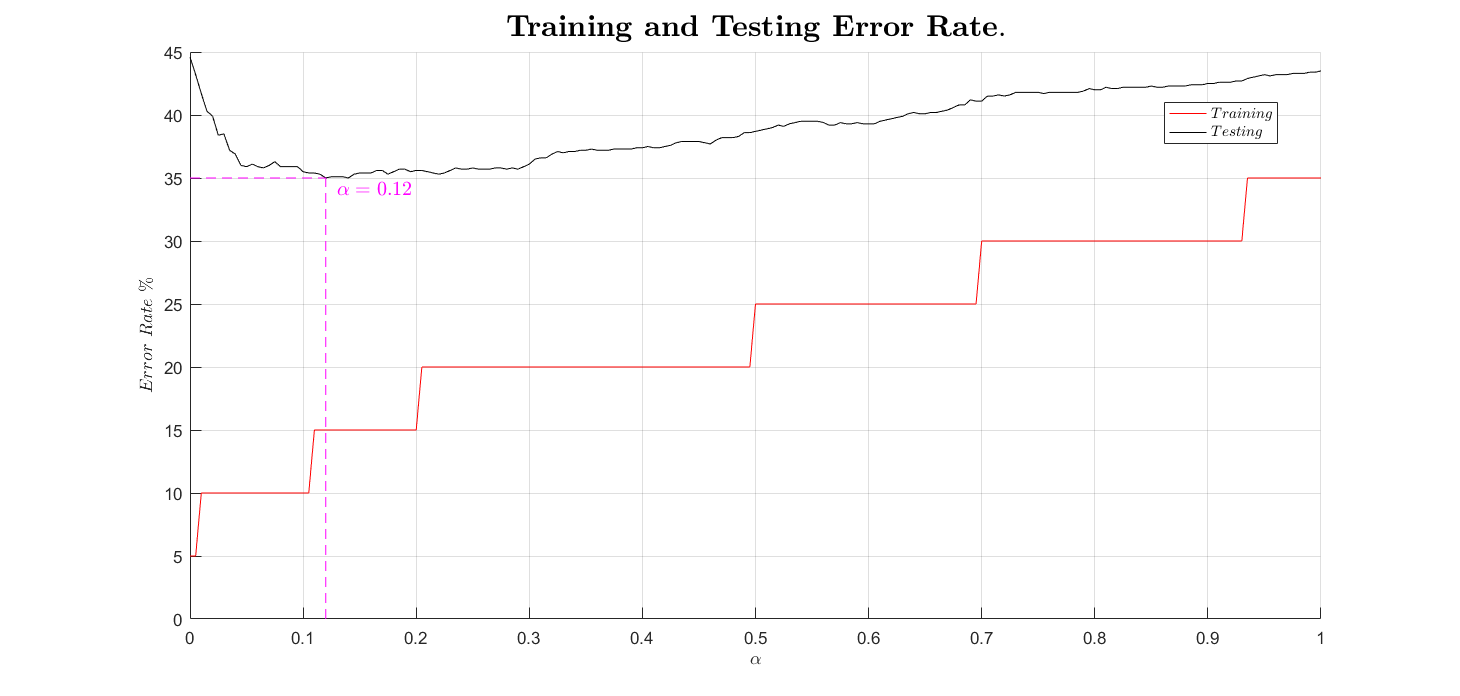
\includegraphics[width = 1\textwidth]{1bc.png}
\caption{Training\ and\ testing\ error\ versus $\alpha$ from\ 0\ to\ 1}
\end{figure}

\noindent(d) With MATLAB the maximum likelihood estimates for mean and covariances are:
\begin{equation*}
\begin{aligned}
\centering {\begin{matrix}
\hat{\bm{\mu_1}} = \begin{bmatrix}
  -0.0110 \\ 
  0.0054 \\ 
  0.0144 \\ 
\end{bmatrix} &  \hat{\bm{\mu_2}} = \begin{bmatrix}
 0.9931 \\
 4.9504 \\
 -2.9815
\end{bmatrix} & \hat{\bm{\mu_3}} = \begin{bmatrix}
 0.0254 \\
 0.0571 \\
 -0.0778
\end{bmatrix}
\end{matrix}}
\end{aligned}
\end{equation*}

\begin{equation*}
\begin{aligned}
\centering {\begin{matrix}
\hat{\bm{\Sigma}}_1 = \begin{bmatrix}
    3.1963  & -0.7264  &  0.4860 \\
   -0.7264  &  2.7638  &  2.7435 \\
    0.4860  &  2.7435  &  3.7038
\end{bmatrix}
\end{matrix}}
\end{aligned}
\end{equation*}

\begin{equation*}
\begin{aligned}
\centering {\begin{matrix}
\hat{\bm{\Sigma}}_2  = \begin{bmatrix}
    1.0692  & -0.5619  &  0.1870  \\
   -0.5619  &  3.1287  & -0.5232  \\
    0.1870  & -0.5232  &  0.9506
\end{bmatrix}
\end{matrix}}
\end{aligned}
\end{equation*}


\begin{equation*}
\begin{aligned}
\centering {\begin{matrix}
\hat{\bm{\Sigma}}_2  = \begin{bmatrix}
    9.3002  & -5.2652  &  5.2015 \\
   -5.2652  & 10.2951  & -5.0706 \\
    5.2015  & -5.0706  & 12.1647
\end{bmatrix}
\end{matrix}}
\end{aligned}
\end{equation*}

\vfill
\clearpage
\noindent\\(e) (f) In this case, the training dataset is large enough for the model to learn the correct parameters. As we can see in Figure 2, the training error tracks the testing error. $\alpha \approx 0$ yields the best performance since the error rates reach minimum at $\alpha \approx 0$, where the estimated variance matrices are closest to the true ones. With shrinkage we could choose from numerous parameters for the variance matrix with best performance.\\
\begin{figure}[H]
\centering
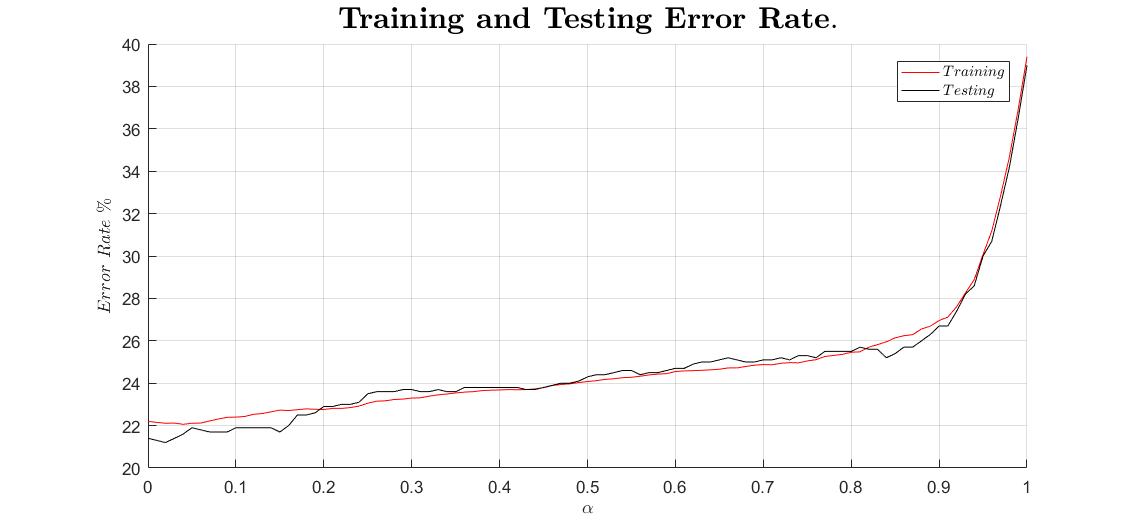
\includegraphics[width = 1\textwidth]{1ef.png}
\caption{Training\ and\ testing\ error\ versus $\alpha$ from\ 0\ to\ 1}
\end{figure}
\text{ }\\
%%---------------------------------------------------------------
%% Problem 2
%%---------------------------------------------------------------
\section{Problem 3.2}
\large{\textbf{Solution:}}\\
(a) As described in the text, the basic version of the K-means algorithm is:\\
\\
\textbf{K-means clustering Algorithm}\\
1 Begin initialize $n,\ c,\ \bm{\mu}_1,\ \bm{\mu}_2,...,\ \bm{\mu}_c$\\
2 Do classify $n$ samples according to nearest $\bm{\mu}_i$\\
3 Recompute $\bm{\mu}_i$\\
4 Until no change in $\bm{\mu}_i$\\
5 Return $\bm{\mu}_1,\ \bm{\mu}_2,...,\ \bm{\mu}_c$\\
6 End\\
\vfill
\clearpage

(b) See Figure 3.
\begin{figure}[H]
\centering
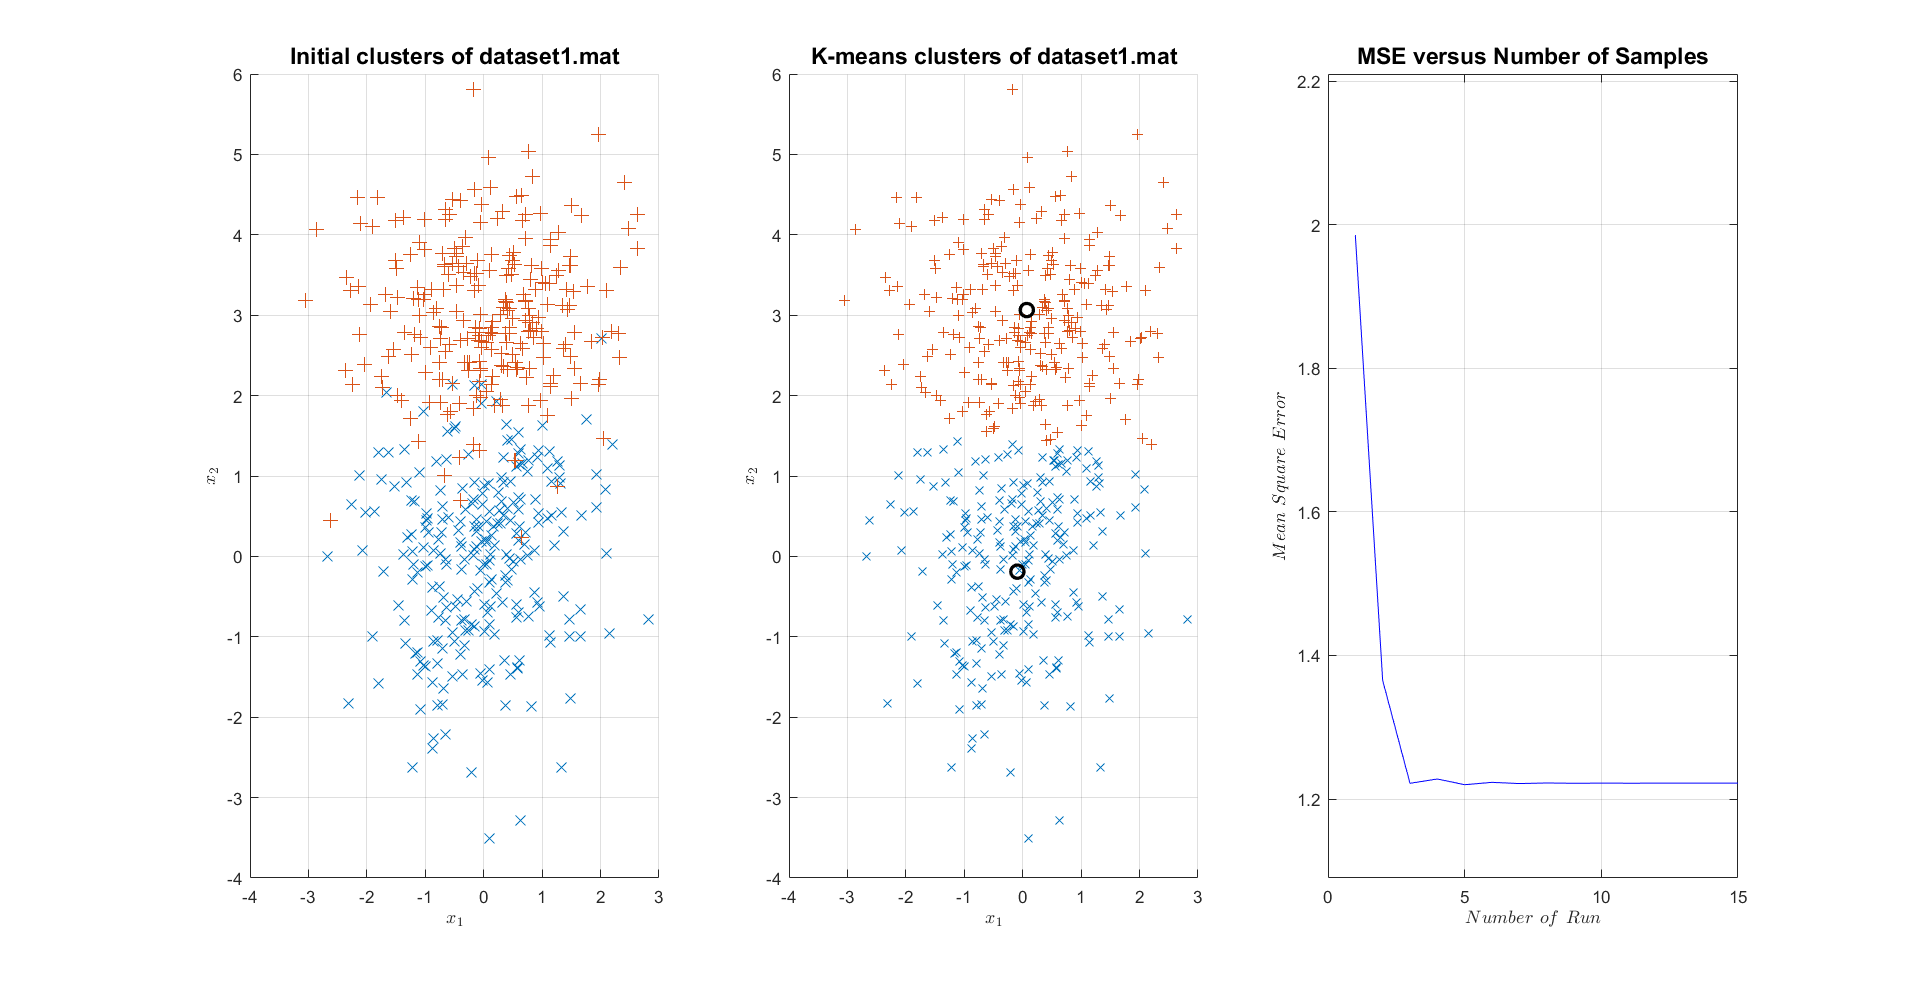
\includegraphics[width = 1\textwidth]{ds1.png}
\caption{Result of clustering with k-means on dataset1.mat}
\end{figure}

\noindent(c) See Figure 4. Since k-means clustering is based on the assumption that all clusters have equal identity covariance matrices, it cannot classify the mixture ellipse dataset to their original shapes.
\\

\begin{figure}[H]
\centering
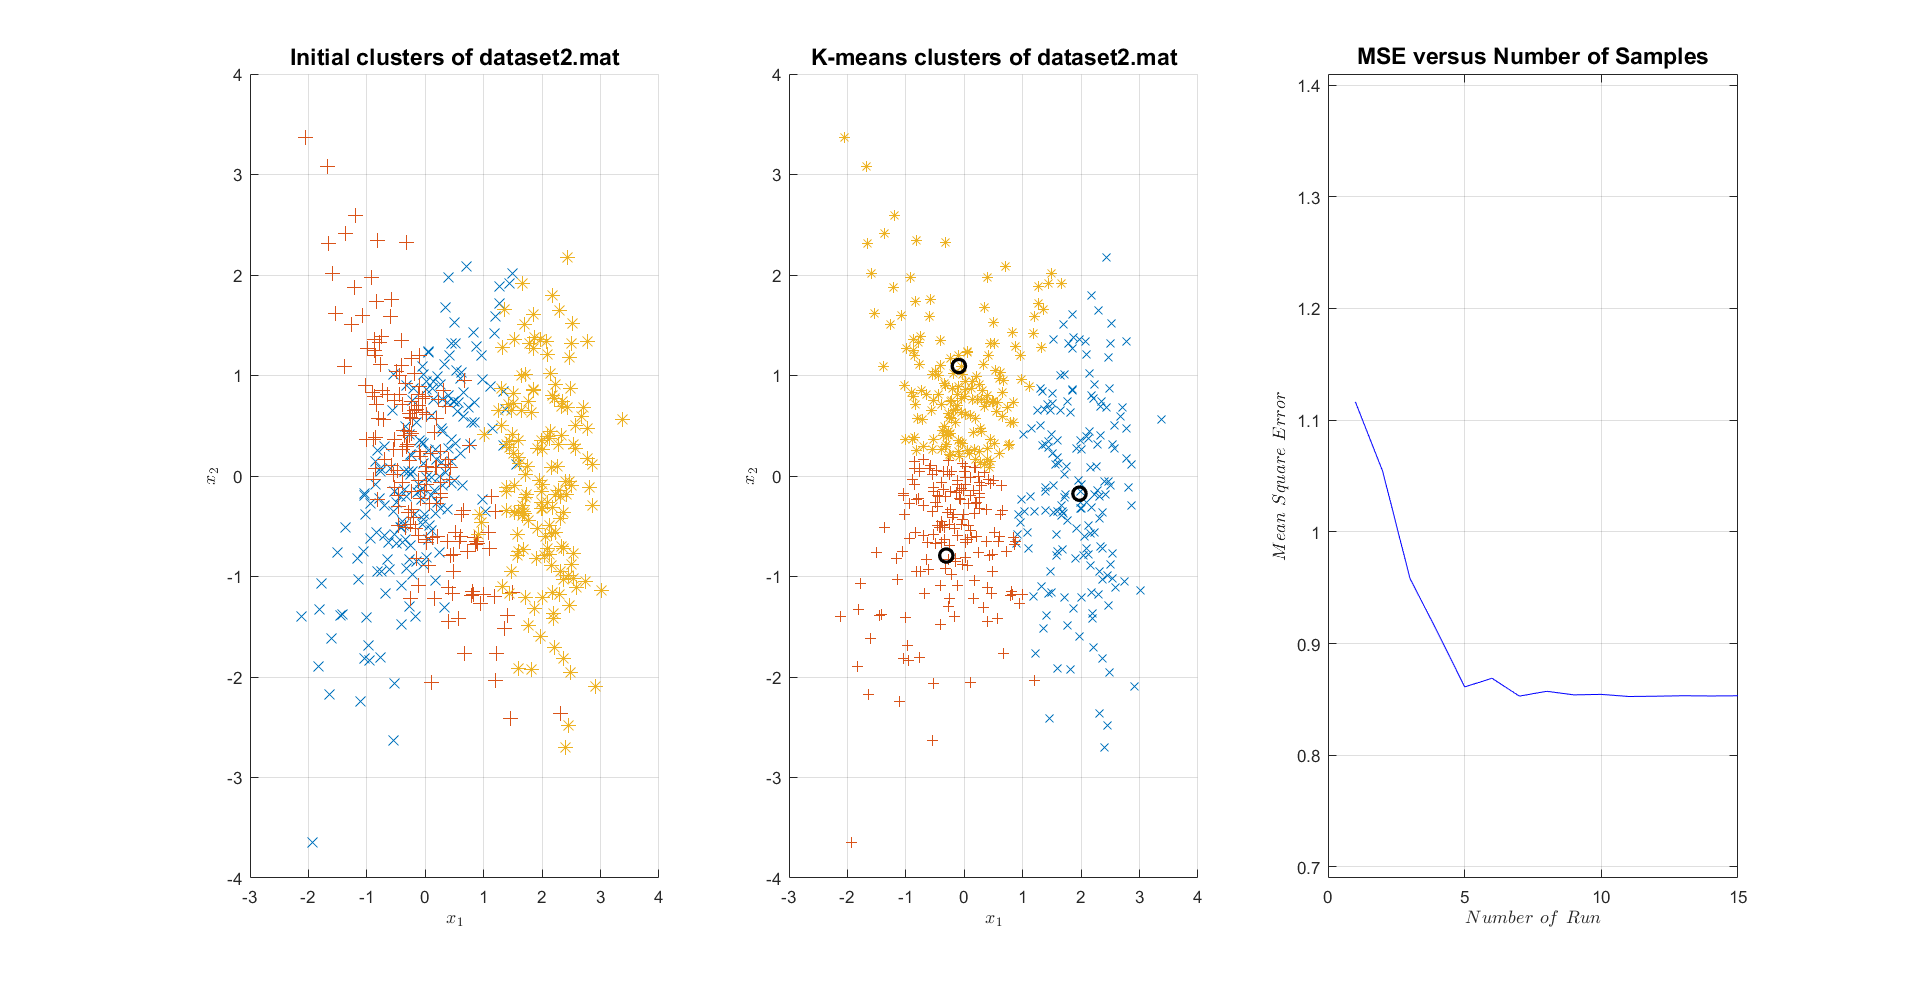
\includegraphics[width = 1\textwidth]{ds2.png}
\caption{Result of clustering with k-means on dataset2.mat}
\end{figure}

\vfill
\clearpage
\noindent(d) See Figure 5.
\begin{figure}[H]
\centering
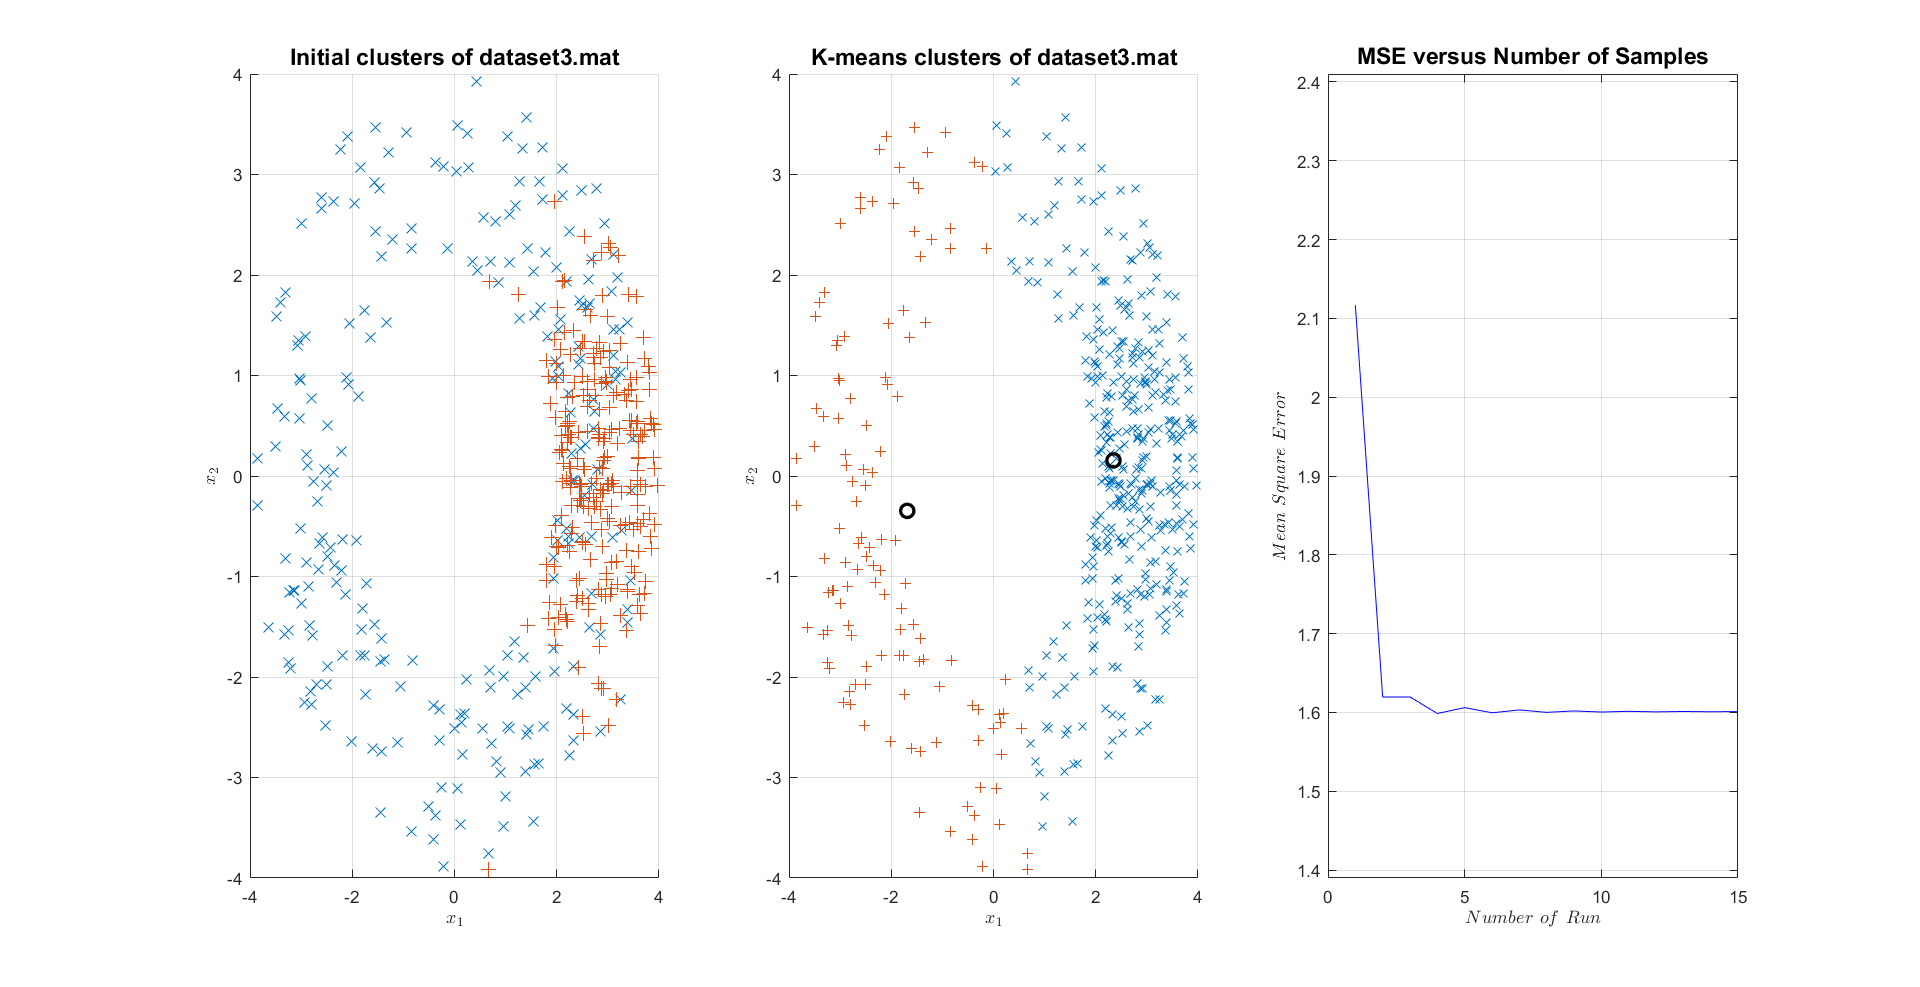
\includegraphics[width = 1\textwidth]{ds3.png}
\caption{Result of clustering with k-means on dataset3.mat}
\end{figure}

\noindent(e) See Figure 6.


\begin{figure}[H]
\centering
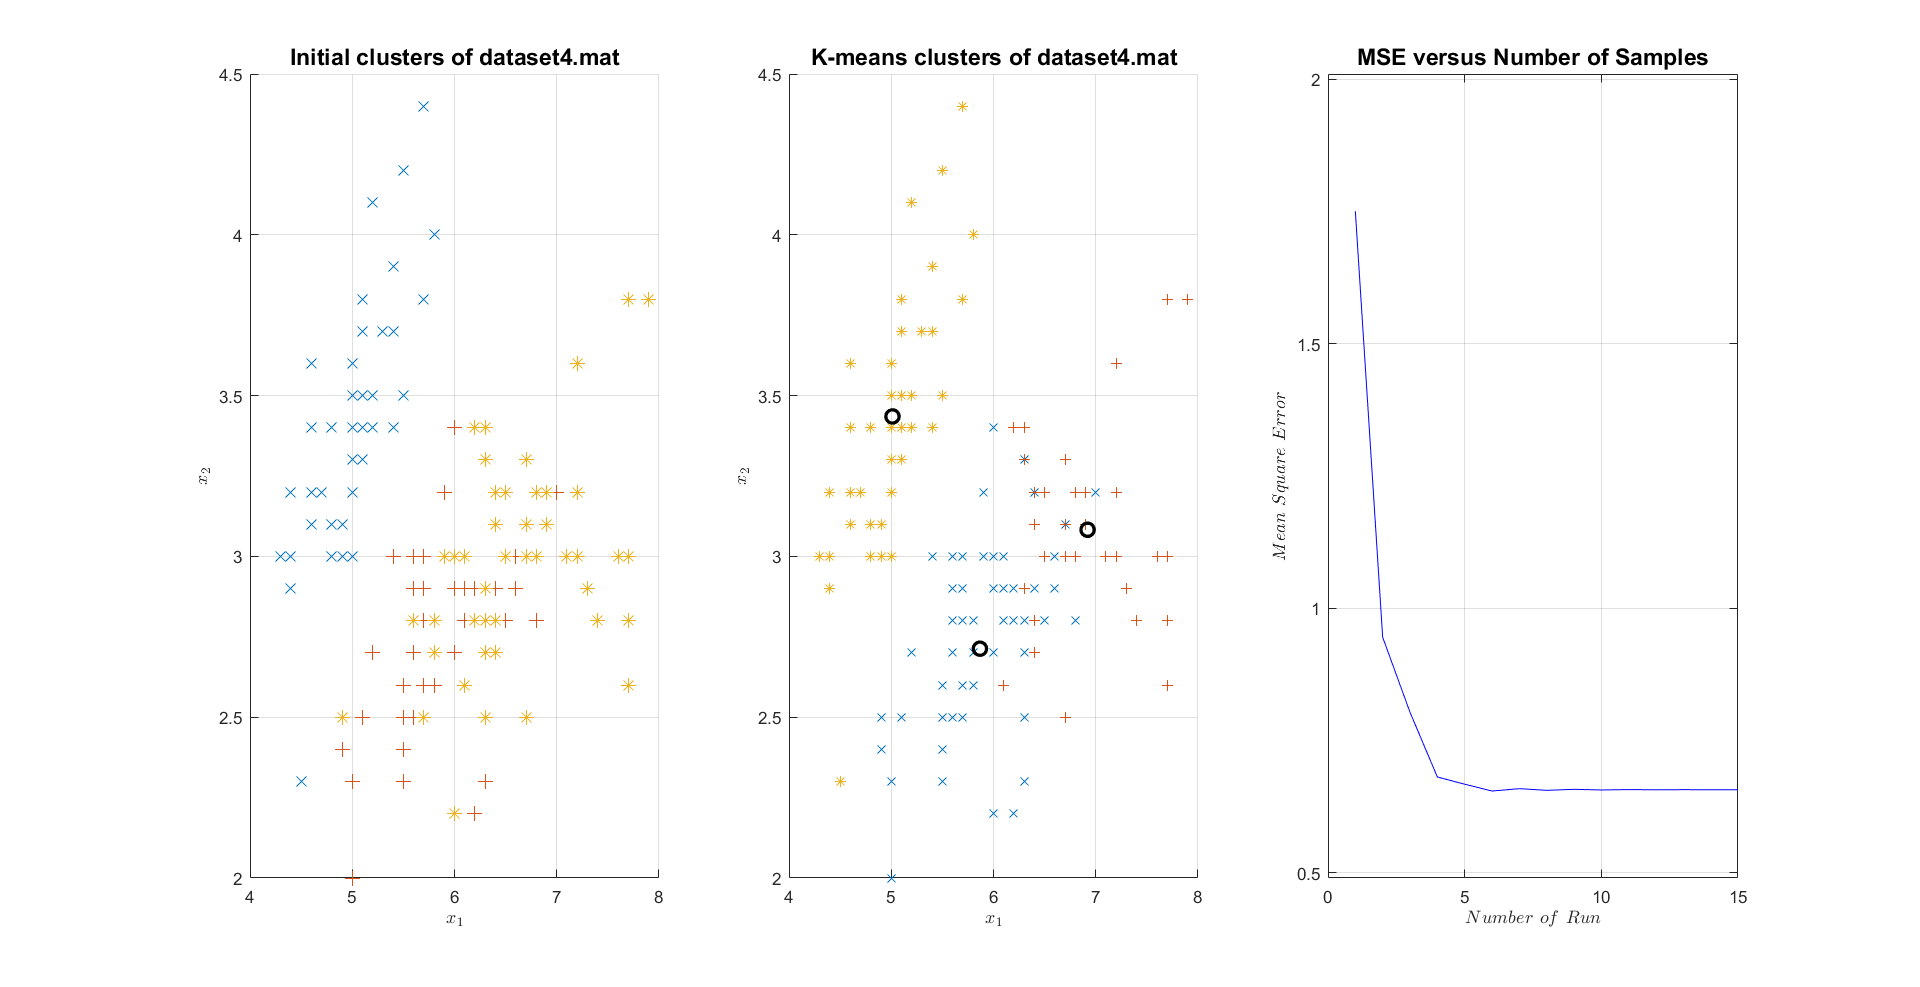
\includegraphics[width = 1\textwidth]{ds4.png}
\caption{Result of clustering with k-means on dataset4.mat}
\end{figure}

\vfill
\clearpage
(f) Knee occurs around $K = 4$

\begin{figure}[H]
\centering
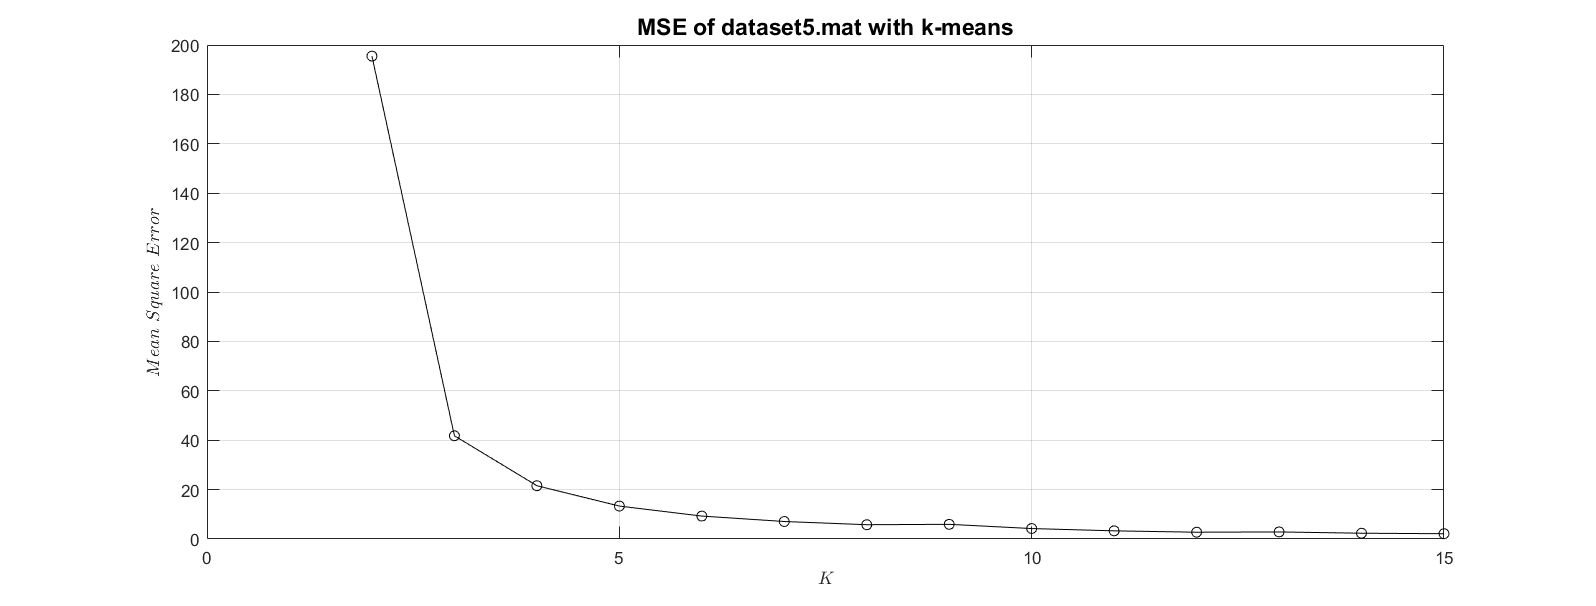
\includegraphics[width = 1\textwidth]{ds5.png}
\caption{MSE of dataset5.mat with k-means}
\end{figure}

\begin{figure}[H]
\centering
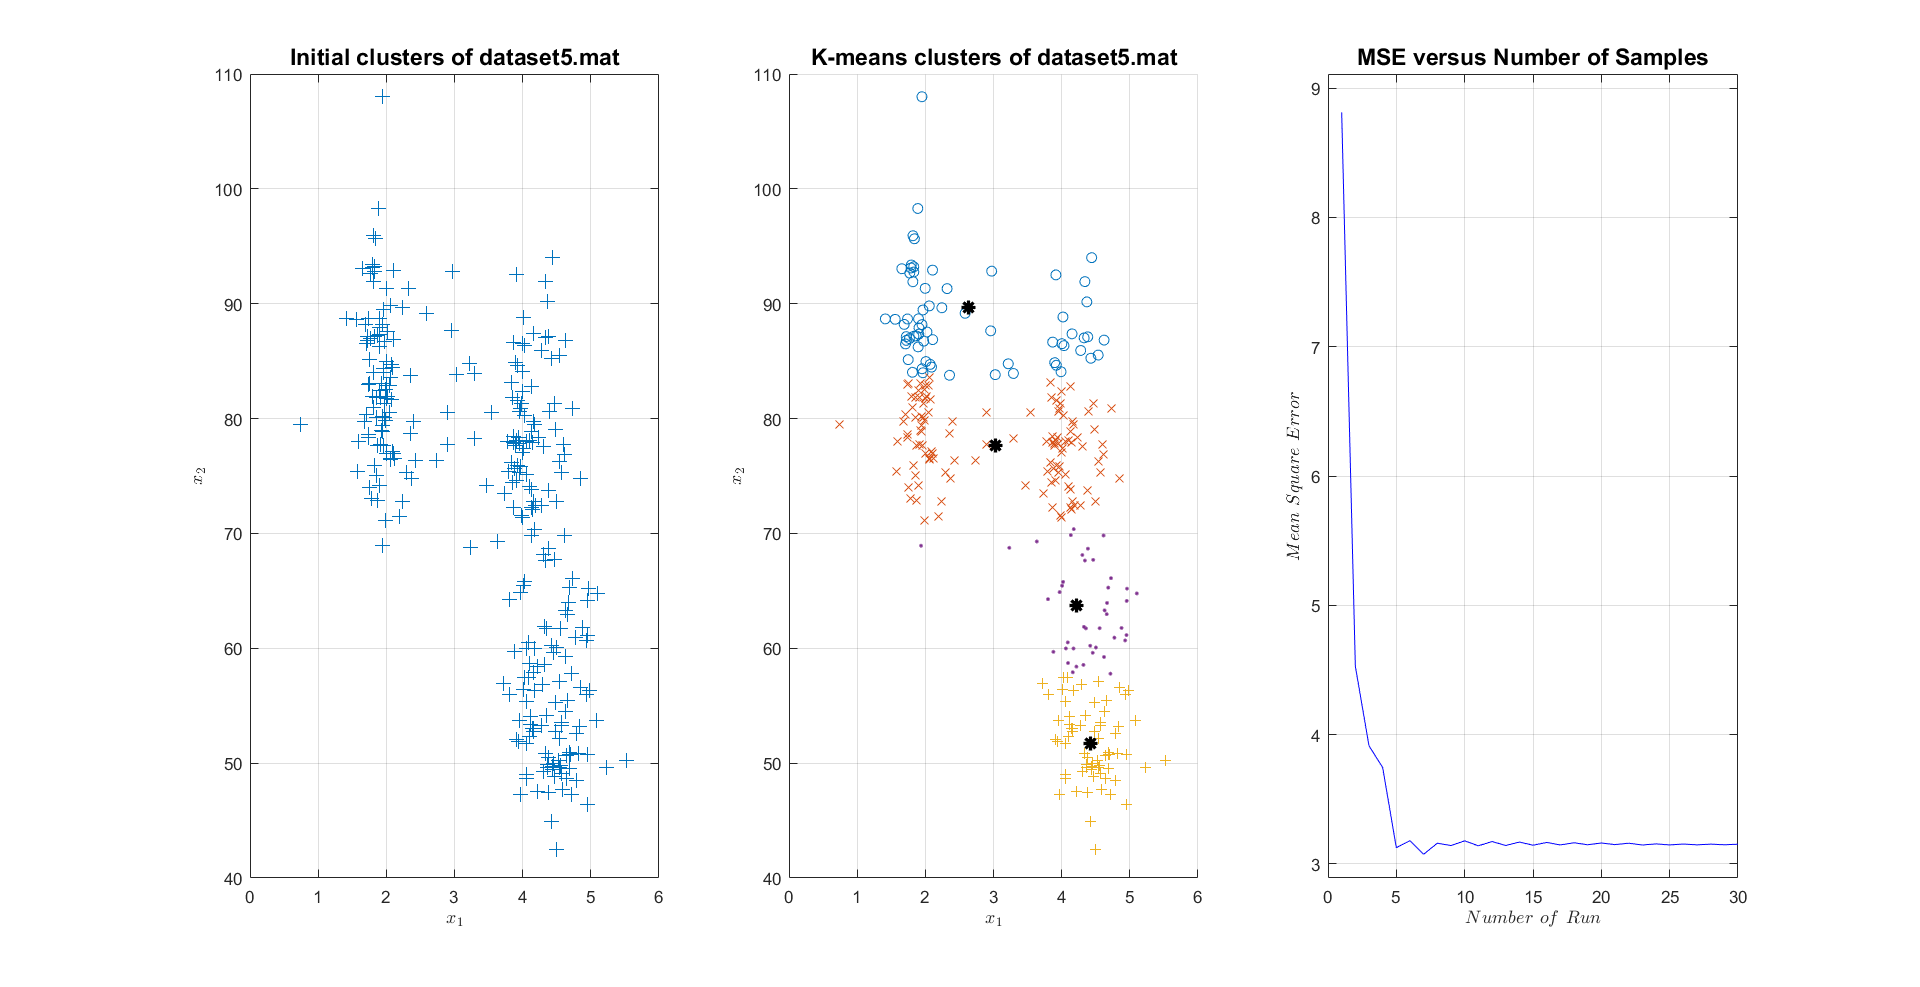
\includegraphics[width = 1\textwidth]{ds52.png}
\caption{Result of clustering with k-means on dataset5.mat}
\end{figure}










\end{document}
